%!TEX root=index.tex
\newacronym{aws}{AWS}{Amazon Web Services}
\newacronym{cpu}{CPU}{Central Processing Unit}
\newacronym{ec2}{EC2}{Elastic Compute Cloud}
\newacronym{iaas}{IaaS}{Infrastructure as a Service}
\newacronym{raid}{RAID}{Redundant Array of Independent Disk}
\newacronym{s3}{S3}{Simple Storage Service}
\section{Reference Big Data Framework}
A framework for data processing has responsibility for achieving several overall goals. These goals, independent from their technical implementation, are a core part of transforming information from raw data to actionable results, such as ClimatEdge\index{ClimatEdge} proposes to provide by giving insurance underwriters probabilities associated with catastrophic events. Applying a big data\index{big data} label means the framework operates at the scale necessary to accommodate the velocity, volume, and variety of expected data. In order to quantitatively process the ever increasing amounts of structured and unstructured data sets necessary in a ClimatEdge\index{ClimatEdge} offering, a technical framework capable of providing the following functionality is needed:
\begin{itemize}
	\item retrieving data updates
	\item storing and indexing for optimal retrieval
	\item data discovery and analytics
	\item presenting real-time and offline results
\end{itemize}
Each functional layer can be represented graphically, building on the layer to its left and on top of an infrastructure implementation. The difference between a framework and a platform is one of flexibility and customization. In order to support a variety of future data types and analytic requirements, a framework of tools is preferable to an extensible platform. Using a framework, it is possible to build loosely coupled layers that can be swapped out as technology evolves and requirements change. While capable of delivering a flexible and extensible solution, the cost of this approach is in the systems integration and development expertise necessary in wiring the layers together in a seamless fashion. Having a framework capable of providing this functionality is crucial in allowing ClimatEdge\index{ClimatEdge} to deliver its offerings to both current and future clients. Figure \ref{layers} shows the layers of the proposed framework.
\begin{figure}[!htbp]
    \centering
    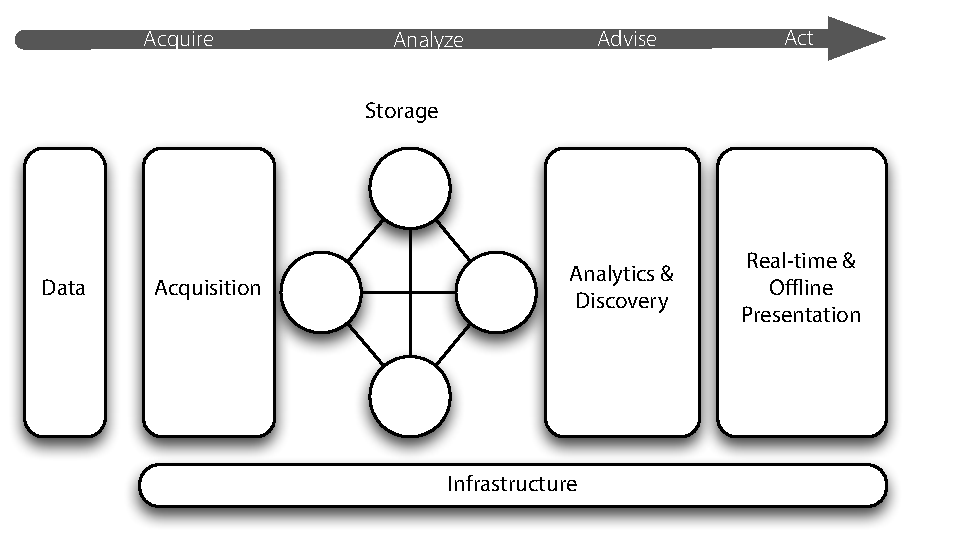
\includegraphics[scale=.62]{framework_layers}
    \caption{Framework layers}
    \label{layers}
\end{figure}
\subsection{Infrastructure}
At the heart of any big data\index{big data} platform is the elastic infrastructure upon which it is built. The concept of both vertical and horizontal elasticity allows the scaling or shrinking of both storage and processing capacity to meet performance requirements and cost efficiency. One method of doing this involves hardware virtualization \index{virtualization} of storage, memory and cpu resources into logical pools that can be assigned or released by services in a pay-per-use model. This allows the various services to acquire more disk space during data ingestion or to request more processors during analytic runs. \textsc{CSC's} BizCloud\index{BizCloud} is a commercial offering built on VMWare \index{VMWare} technology that allows elastic \gls{iaas}\index{IaaS} for its customers \cite{bizcloud}. Two \gls{iaas} technologies popular with both startups and Internet companies such as Netflix\index{Netflix}, are part of the \gls{aws}\index{AWS} stack: the Xen\index{Xen} based \gls{ec2}\index{EC2} and the \gls{s3}\index{S3} \cite{cockcroft}. \gls{ec2} is used for any computing, regardless of elasticity, while \gls{s3} is used as simple object storage. Regardless of the specific technology used, the infrastructure layer has two fundamental requirements:
\begin{itemize}
    \item cost effectiveness in horizontal scaling
    \item ease of adding, requesting, relinquishing resources
\end{itemize}
Missing from the above list is reliability. Many industry leaders, such as Google\index{Google}, Amazon\index{Amazon}, Netflix\index{Netflix}, Twitter\index{Twitter}, etc, have implemented reliability in software as opposed to hardware, effectively moving it into the software storage layer. This approach gives the flexibility to completely replace failed storage and compute nodes with upgraded versions at leisure and without necessarily impacting overall reliability. This also has the added benefit of  reducing hardware storage costs, since expensive \gls{raid} technology is no longer required to be purchased during every technology refresh.\\

As offerings mature and new capabilities are brought online, it is probable that certain data sets outside of ClimatEdge\index{ClimatEdge}, such as healthcare, may want to be kept within corporate control to ease privacy concerns. In this situation, a platform built on \gls{aws}\index{AWS} is not feasible. While BizCloud\index{BizCloud} is currently the preferred corporate solution, an open source based platform could also be created which replicates best practices from other big data\index{big data} organizations. Facebook's\index{Facebook} Open Compute Project\index{Open Compute Project} is a community targeted hardware effort in data center efficiency, with many vendors selling compliant solutions \cite{opencompute}. Combined with a hypervisor such as Xen\index{Xen} \cite{xen} or a cloud solution like OpenStack\index{OpenStack} \cite{openstack}, it is possible to replicate \gls{iaas}\index{IaaS} functionality in house through open source.
\subsection{Data Acquisition}
The data acquisition layer holds the technology to retrieve the latest data sets, pre-process them with parsers  to extract the required information and pass them onto the storage and indexing layer for permanent storage. By definition, this layer has a basic requirement of storage and compute elasticity. As an example, the \gls{merra} data sets can be upwards of forty terabytes when taking into account all the variables. However, certain analytics require much fewer variables than what is included in the default collections. It is possible to simply store all of the variables in hopes that future offerings can make use of them or they can be discarded in order to save storage space. A 300 megabyte daily file might be reduced to 30 megabytes after extraneous variables are discarded. In order to ingest the entire thirty-three year \gls{merra} history in chunks, three to four terabytes would  temporarily be required. However the information indexed and persistently stored might be closer to 300 or 400 gigabytes. Along similar lines, one \gls{cpu} core might be allocated to process each year of data in parallel for speed, requiring thirty-three simultaneous cores for a short period of time. \\

The technical implementation of a process to retrieve data at pre-defined intervals is a relatively simple systems integration and development task and has plenty of prior art across the industry. The following components can be used to accomplish this task:
\begin{itemize}
	\item Linux instances to handle retrieval, parsing, monitoring, and hosting the source code repository, respectively. Note that the number of associated cores and instances may vary from the time historical loads are performed to when new data is added.
	\item A continuous integration tool, Jenkins\index{Jenkins} or similar, for monitoring and notifying the success or failure of the retrieval processes (one notification per data set). Jenkins will also serve as the means to deploy the most recent code from the code repository onto the server handling the retrieval process. Jenkins is open source and commonly used across the industry for this purpose, resulting in an easily hirable skill set \cite{jenkins}.
	\item A repeatable method, such as Cron, to check and retrieve updated data sets at well defined publication intervals. Jenkins will monitor the success or failure of the cron jobs and notify as needed. Jenkins is also capable of implementing repeatable tasks natively.
	\item Developed code that contacts each data source and pulls down only the most recent data. If the data sets do not offer a simple means of determining what is recent, the code can query the local data store so that it is aware of the most recently stored data and download appropriately. While unique code is needed for each data set, the process of determining what is new and retrieving the code is generally similar across data sets. It is likely there will be a reusable library of common functionality shared across each specific implementation. This development is likely to be done in a scriptable environment such as Python or Perl, as the languages offer an excellent tradeoff between simplicity, flexibility, and execution speed.
\end{itemize}
\subsection{Storing and Indexing}
 The heart of any data processing framework is the means by which data is stored and indexed for retrieval. Depending on the particular implementation, this layer can also replicate data for availability, though it is not viewed as a firm requirement. Any implementation choice should support the following characteristics:
\begin{itemize}
	\item not inherently possess a single point of failure
	\item horizontally scale (as linearly as possible) in both storage and performance
	\item support indexing and retrieval for both real-time and offline analytics
\end{itemize}
The top level Apache Hadoop project houses technologies which fulfill the requirements listed above, one being Cassandra\index{Cassandra}, which is supported by companies like DataStax\index{DataStax} \cite{cassandra}. There are competing technologies from commercial vendors like EMC\index{EMC}, IBM\index{IBM}, Intel\index{Intel}, SAS\index{SAS}, and Oracle\index{Oracle} just to name a few, that have similar technologies designed to store and index vast amounts of data. If data replication was not implemented natively in the underlying hardware infrastructure layer, it is absolutely crucial that it is implemented here by the storage software. As with any data replication implementation, proper capacity planning must be performed to ensure that space is available for both the initial data load and the predicted growth.\\

In terms of logical representation inside of a data store, table \ref{model} lists a generic key-value model for any piece of climate data. It is suitable for any column oriented solution, but is easily adapted to a traditional row-based technology, such as Oracle Enterprise\index{Oracle} or MySQL\index{MySQL}.
\begin{table}[htbp]
    \centering
    \begin{tabular}{l l}
        \hline
	Key & Value \\ [0.5ex]
	%heading
	\hline
	meta-data & what the measurement represents, e.g., total precipitation or soil moisture\\
	time & time and date of measurement in UTC, e.g., YYYY-MM-DD HH:MM:SS\\
	coordinates & geographic location in latitude and longitude, e.g. -90.0 to 90.0 and -180.0 to 180.0\\
	value & measurement value, e.g. 0.000052977\\
	\hline
    \end{tabular}
    \caption{Climate Data Model}
    \label{model}
\end{table}
This simple structure, in conjunction with materialized views,\index{materialized views} enables fast analytic retrieval of data based on any combination of the following: temporal, geospatial, or by meta-data. Materialized views provide an alternative to traditional indexing technology that work well, but at the cost of storage efficiency \cite{materialized_views}. 
\subsection{Discovery and Analytics}
The technology behind big data\index{big data} storage is generally only interesting to engineers. Customers pay for the results and insights gleaned from analysis of the stored data. The discovery and analytic processes make further usage of the elastic compute infrastructure identified earlier. Analytics can generally be organized into the two modes in which they are run: real-time and offline. Whenever analytics are run, it is crucial to design the algorithms to take advantage of additional capacity as needed and then to release it to realize cost savings. Through extensive testing and modeling, it should be straightforward to estimate the necessary capacity for all the offline analytics and spin up resources at well established intervals. Real-time is somewhat more complex as it is difficult to understand capacity requirements a priori. Analytical implementations vary according to specific requirements, but R, Java, and Python are extremely popular analytic implementation languages and would be ideal for ClimatEdge\index{ClimatEdge} offerings. Commercial discovery and analytics solutions that work with multiple storage technologies, such as Instaview\index{Instaview}, are much more flexible than products that ship with their own storage layer \cite{pentaho}. This flexibility allows solutions which combine the optimal storage layer to the analytic layer without having to reinvent the wheel. Both classes of analytics are presented in further detail below.
\subsubsection{Offline Analytics}
Offline analytics, also known as batch, are run at predefined intervals without human interaction. Well defined questions are implemented ahead of time, optimized in the storage layer, tested and refined, and then set to run through a scheduling mechanism like Jenkins\index{Jenkins} or Cron. The tornado and flood analytics are excellent examples of batch jobs needing to be run at well defined intervals to take account of updated data. MapReduce\index{MapReduce}, popularized by Google\index{Google}, is an extremely common implementation of distributed processing over large data sets. It is implementation agnostic and several popular frameworks exist to speed up development. The output from the MapReduce\index{MapReduce} jobs can be written to the data store and used as input to the presentation layer.
\subsubsection{Real-time Analytics}
Real-time analytics are run on demand, though implementations should make use of as much precomputed data as possible for execution speed. Since it is not feasible to understand every possible data combination or question in advance, the focus should be on optimizing commonly accessed data. For example, gathering totals, averages, or means over a time period so it is available on demand as a lookup would optimize retrieval time. The tradeoff is between storage used and speed of execution. In most cases, real-time analytics are launched by users and the framework is well served by returning answers as quickly as possible, even at the cost of additional storage.\\

One approach to real-time analytics involves crowd sourcing. Conceptually simple, the trick lies in implementing it correctly. Essentially, any time a real-time analytic is run, the data is turned into a repeatable offline analytic behind the scenes. This particular analytic can then be presented to the user as one that has been precomputed, thus saving time. For example, if the average rainfall was desired for a particular latitude and longitude, an offline analytic could be created that precomputes this value once per month. Over time, the goal is to change as many real-time questions as possible into precomputed answers.
\subsection{Presentation}
The presentation layer not only handles delivery of both types of analytic results, but also handles any user interaction with the data store, such as interactive discovery or real-time queries. While each and every business offering has specific requirements in terms of what is delivered and how it is presented, several tools can ease the burden of developing custom solutions for each offering. Data visualization, usually graphical in nature, is a specific instance of information presentation and can be assumed to be handled within this layer. Discussions were conducted with the sales team at Quantum4D around their main data discovery and visualization product \cite{quantum}. While there are many products that provide similar capabilities, the Quantum4D platform is storage layer agnostic which stands out amongst its competitors and makes an excellent addition to the presentation layer.\\

At the highest level, any modern framework should support the following formats, as they will cover many of the use cases: \gls{html}, mobile, and structured text. Fortunately, wide adoption of \gls{html}5 standards across both desktop and mobile browsers brings the promise of "write once, run anywhere" closer to fruition. However, mobile applications that require advanced security and graphically intensive user experiences will benefit from native implementation in either Objective-C\footnote{Apple iOS} or Java\footnote{Google Android}. Structured text is often represented by serialized \gls{xml}, as is the case with ClimatEdge\index{ClimatEdge} offerings. Customer specific implementations are often required in any offering, which leads to presentation solutions built upon various Javascript\index{Javascript} libraries such as Node.js, Socket.io, Processing.js and Backbone.js.
\subsection{Effective Framework Keys}
The components presented here are one implementable approach to a flexible big data\index{big data} framework for ingesting, storing, analyzing, and presenting both structured and unstructured data. There is no commercial solution capable of covering every possible scenario. Since requirements evolve and technologies improve, today's solution may not work tomorrow and tomorrow's solution may not exist yet. Therefore, a flexible and loosely coupled framework capable of containing a variety of technologies is a superior approach that will allow \textsc{CSC} to choose the most efficient tool for each offering. By utilizing a set of interconnected and agnostic technologies in each layer, the solution framework and expertise \textsc{CSC} is investing in today will fit the customers and requirements of tomorrow.
